%----------------------------------------------------------------------------------------
%	PACKAGES AND OTHER DOCUMENT CONFIGURATIONS
%----------------------------------------------------------------------------------------

\documentclass[a4paper,10pt]{memoir} % Font and paper size

%%%%%%%%%%%%%%%%%%%%%%%%%%%%%%%%%%%%%%%%%
% Wenneker Resume/CV
% Structure Specification File
% Version 1.1 (19/6/2016)
%
% This file has been downloaded from:
% http://www.LaTeXTemplates.com
%
% Original author:
% Frits Wenneker (http://www.howtotex.com) with extensive modifications by 
% Vel (vel@latextemplates.com)
%
% License:
% CC BY-NC-SA 3.0 (http://creativecommons.org/licenses/by-nc-sa/3.0/)
%
%%%%%%%%%%%%%%%%%%%%%%%%%%%%%%%%%%%%%%%%%

%----------------------------------------------------------------------------------------
%	PACKAGES AND OTHER DOCUMENT CONFIGURATIONS
%----------------------------------------------------------------------------------------

% \usepackage{XCharter} % Use the Bitstream Charter font
\usepackage[default,scale=0.95]{opensans}
\usepackage[utf8]{inputenc} % Required for inputting international characters
\usepackage[T1]{fontenc} % Output font encoding for international characters
\usepackage[none]{hyphenat} % Disable hyphenation
\usepackage{multicol}
\usepackage{hyperref}
\usepackage{cfr-lm}
\usepackage{ifthen}


\usepackage[top=1cm,left=0.7cm,right=0.7cm,bottom=1cm]{geometry} % Modify margins


\usepackage{graphicx} % Required for figures

\usepackage{flowfram} % Required for the multi-column layout

\usepackage{url} % URLs

\usepackage[usenames,dvipsnames]{xcolor} % Required for custom colours

\usepackage{tikz} % Required for the horizontal rule

\usepackage{enumitem} % Required for modifying lists
\setlist{noitemsep,nolistsep} % Remove spacing within and around lists
\setlist[itemize]{leftmargin=*}

\setlength{\columnsep}{\baselineskip} % Set the spacing between columns

\urlstyle{sf}

% Define the left frame (sidebar)
\newflowframe{0.2\textwidth}{\textheight}{0pt}{0pt}[left]
\newlength{\LeftMainSep}
\setlength{\LeftMainSep}{0.2\textwidth}
\addtolength{\LeftMainSep}{1\columnsep}
 
% Small static frame for the vertical line
\newstaticframe{1.5pt}{\textheight}{\LeftMainSep}{0pt}
 
% Content of the static frame with the vertical line
\begin{staticcontents}{1}
\hfill
\tikz{\draw[loosely dotted,color=RoyalBlue,line width=1.5pt,yshift=0](0,0) -- (0,\textheight);}
\hfill\mbox{}
\end{staticcontents}
 
% Define the right frame (main body)
\addtolength{\LeftMainSep}{1.5pt}
\addtolength{\LeftMainSep}{1\columnsep}
\newflowframe{0.7\textwidth}{\textheight}{\LeftMainSep}{0pt}[main01]

\pagestyle{empty} % Disable all page numbering

\setlength{\parindent}{0pt} % Stop paragraph indentation

%----------------------------------------------------------------------------------------
%	NEW COMMANDS
%----------------------------------------------------------------------------------------

\newcommand{\userinformation}[1]{\renewcommand{\userinformation}{#1}} % Define a new command for the CV user's information that goes into the left column

\newcommand{\cvheading}[1]{{\Huge\bfseries\color{RoyalBlue} #1} \par\vspace{.6\baselineskip}} % New command for the CV heading
\newcommand{\cvsubheading}[1]{{\Large\bfseries #1} \bigbreak} % New command for the CV subheading

\newcommand{\Sep}{\vspace{1em}} % New command for the spacing between headings
\newcommand{\SmallSep}{\vspace{0.5em}} % New command for the spacing within headings

\newcommand{\aboutme}[2]{ % New command for the about me section
\textbf{\color{RoyalBlue} #1}~~#2\par\SmallSep
}
	
\newcommand{\CVSection}[1]{ % New command for the headings within sections
\SmallSep
{\Large{\textbf{#1}}}\par\SmallSep % Used for spacing
}



% Parameters
% #1: Company
% #2: Position
% #3: Location
% #4: Date
% #5: Link
% #6: Description
\newcommand{\CVItem}[6]{ % New command for the item descriptions
\CreateTitle{#1}{#2}{#5}{#3} \Date{#4} \par\SmallSep
#6
\InsertSmallSepIfNonEmpty{#6}
}

\newcommand{\Date}[1]{
\hfill{ \small{\textcolor{CadetBlue}{\textit{\sbweight{#1}}}} }
}

\newcommand{\DateLocation}[2]{
\hfill{{\small  \textcolor{CadetBlue}{\sbweight{#2} \hspace*{2pt}} \textit{#1}} }
}


\newcommand{\InsertSmallSepIfNonEmpty}[1]{
    \if\relax\detokenize{#1}\relax
        % Empty
    \else
        % Non-empty
        \par\SmallSep
    \fi
}

% Parameters
% #1: Location
% #2: Description
\newcommand{\InsertLocation}[2]{
    \if\relax\detokenize{#1}\relax
        \par\SmallSep
        #2
    
    \else
        \par
        \hspace*{\fill}{\small\textit{#1}}
        \par\SmallSep
        #2
    \fi
}


% Parameters
% #1: Title
% #2: Position
% #3: Link
% #4: Location
\newcommand{\CreateTitle}[4]{
    \if\relax\detokenize{#2}\relax
        \textbf{\color{RoyalBlue} \link{#3}{#1}}
    \else
        \textbf{\color{RoyalBlue} \link{#3}{#1, \textit{#2}}} 
    \fi
    \if\relax\detokenize{#4}\relax
    \else
        \hspace*{3pt} \textit{#4}
    \fi
}

% Parameters
% #1: Module
% #2: Mark
\newcommand{\Module}[2]{
    \bluebullet #1 \hspace*{2pt}{\small\textit{(#2\%)}}
}

% Same as module, without the %
\newcommand{\ALevel}[2]{ 
    \bluebullet #1 \hspace*{2pt}{\small\textit{(#2)}}
}

\makeatletter
\newcommand*{\link}{\begingroup\@makeother\#\@mylink}
\newcommand*{\@mylink}[2]{\href[pdfnewwindow=true]{#1}{#2}\endgroup} 
\makeatother


\newcommand{\bluebullet}{\textcolor{RoyalBlue}{$\circ$}~~} % New command for the blue bullets
 % Include the file specifying document layout and packages

\userinformation{ % Set the content that goes into the sidebar of each page
\begin{center}

%----------------------------------------------------------------------------------------
%	NAME AND CONTACT INFORMATION 
%----------------------------------------------------------------------------------------

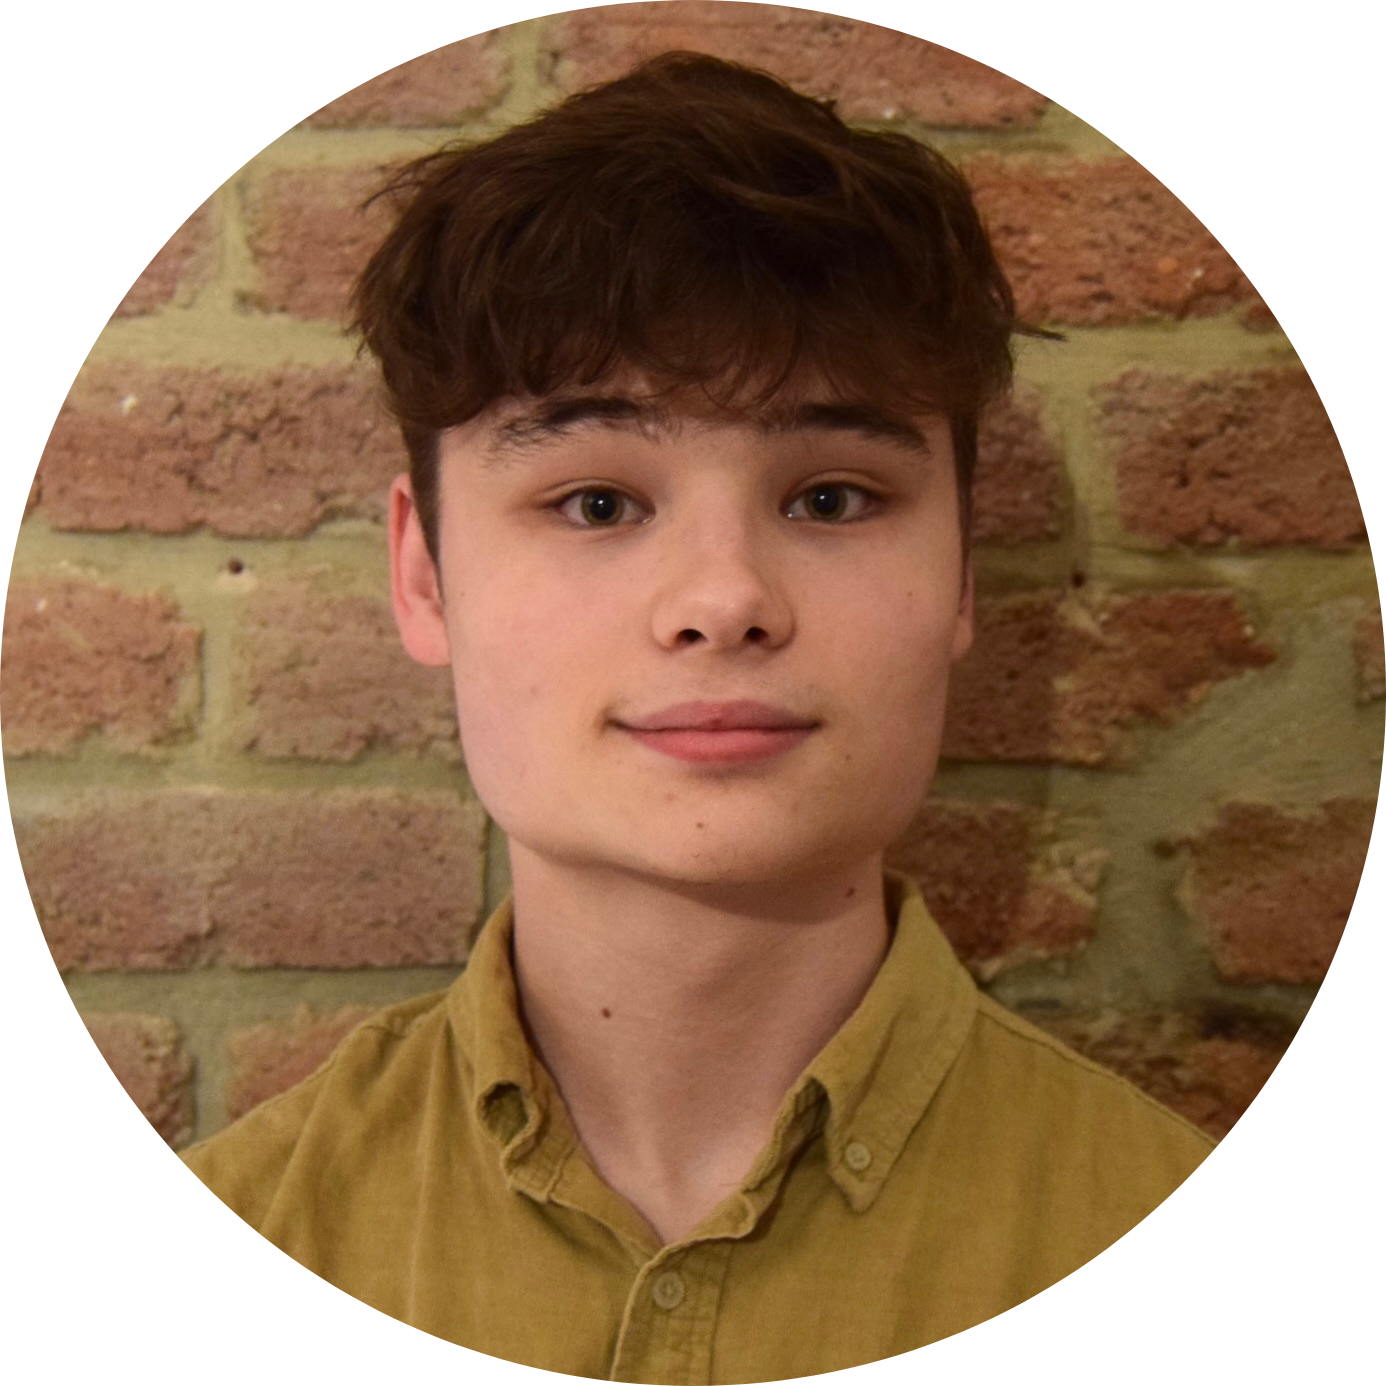
\includegraphics[width=0.75\columnwidth]{portrait.png}\\[\baselineskip]
\small % Smaller font size for left column
\link{mailto:tcp510@york.ac.uk}{tcp510@york.ac.uk} \\
(+44) 77400 54268 \\ % Your phone number
York, UK \\
\Sep

\link{https://tompollak.me}{tompollak.me} \\
\link{https://github.com/tom-pollak}{github.com/tom-pollak} \\
\Sep

%----------------------------------------------------------------------------------------
%	LANGUAGES, TECHNOLOGIES, AND INTERESTS
%----------------------------------------------------------------------------------------

\textbf{Languages} \\
\SmallSep
Python, Java, Haskell, JavaScript, SQL, HTML, CSS \\
\Sep

%------------------------------------------------

\textbf{Technologies} \\
\SmallSep
Linux, Git, Vim, testa, Django, Numpy, Pandas, LibGDX, Docker, Vue.js, Selenium \\
\Sep

%------------------------------------------------

\textbf{Interests} \\
\SmallSep
Mountain biking, Climbing, Poker, Chess, Running, Hockey \\
\end{center}
\vfill % Whitespace under this block to push it up under the photo
}

%----------------------------------------------------------------------------------------

\begin{document}

\userinformation % Print your information in the left column

\framebreak % End of the first column

%----------------------------------------------------------------------------------------
%	HEADING
%----------------------------------------------------------------------------------------

\cvheading{Tom Pollak} % Large heading - your name

\cvsubheading{CS Student @ University of York} % Subheading - your occupation/specialization

%----------------------------------------------------------------------------------------
%	ABOUT ME
%----------------------------------------------------------------------------------------

\aboutme{About Me}{
	A second year Computer Science student studying at the University of York
	seeking a summer internship in software development or other related fields.
	I enjoy learning practically, and have developed a number of personal
	projects to further my knowledge in areas that interest me. I am most
	proficient with Python but also have experience in Java and Haskell, with a
	working knowledge of JavaScript. I have many years of experience
	working with Linux systems and Git version control.
}

\SmallSep % Small sep as lms education seems to have weird vertical spacing i cant get rid of

%----------------------------------------------------------------------------------------
%	EDUCATION
%----------------------------------------------------------------------------------------

\CVSection{Education}

%------------------------------------------------

\CVItem{University of York}{}{}{2020 - 2023}{https://york.ac.uk}{
	\textbf{BEng Computer Science} \hspace*{11pt}{\small{\sbweight{\textit{\textcolor{darkgray}{Average 77\%, Expected First}}}}} \\[4pt]
	\begin{tabular}{ p{0.2\textwidth} p{0.2\textwidth} p{0.3\textwidth} }
		\Module{Theory 1}{81} & \Module{Theory 2}{72} & \Module{Theory 3}{78} \\
		\Module{Data 1}{72} & \Module{Data 2}{72.5} & \Module{Intelligent Systems 1}{73} \\
		\Module{Software 1}{95} & \Module{Software 2}{94} & \Module{Systems \& Devices 1}{78} \\
		\Module{\raggedright Human Computer \hspace*{8pt} Interaction 1}{66} &\Module{\raggedright Human Computer \hspace*{8pt} Interaction 2}{70} & \Module{Systems \& Devices 2}{71}
	\end{tabular}
}

%------------------------------------------------

\CVItem{Lady Manners School}{}{Bakewell, UK}{2020}{}{
	\begin{tabular}{p{0.2\textwidth} p{0.2\textwidth} p{0.3\textwidth} }
		\textbf{A-level} & & \textbf{GCSE} \\[2pt]
		\ALevel{Further Maths}{A} & \ALevel{Maths}{A} & \bluebullet 5 8s, 2 7s, 2 6s, 1 5. \\
		\ALevel{Computer Science}{A} & \ALevel{Physics}{A}
	\end{tabular}
}

%----------------------------------------------------------------------------------------
%	EXPERIENCE
%----------------------------------------------------------------------------------------

\CVSection{Experience}

%------------------------------------------------

\CVItem{Cisco Meraki}{Full Stack Engineer Intern}{London, UK}{June 2022 - August 2022}{https://meraki.cisco.com/en-uk/}{}

\SmallSep

%----------------------------------------------------------------------------------------
%	PROJECTS
%----------------------------------------------------------------------------------------

\CVSection{Projects}

%------------------------------------------------

\CVItem{Automated Horse Betting Program}{}{}{December 2020 - July 2021}{https://github.com/tom-pollak/each-way-matcher}{
	Discovers undervalued horses by the bookmaker in each-way betting.
	\vspace*{2pt}\begin{itemize}
		\item Uses an adapted Kelly Criterion strategy to calculate the optimal stake to profit of these undervalued horses.
		\item Runs headless on a Raspberry Pi as a scheduled cron job every day.
	\end{itemize}
}

%------------------------------------------------

\CVItem{Pirate Game}{}{}{January - February 2022}{https://github.com/tom-pollak/pirates}{
	Interactive pirate game using Java and LibGDX.
}

%------------------------------------------------

\CVItem{Poker Web Application}{}{}{April 2019 - July 2020}{https://github.com/tom-pollak/web-poker}{
	Free live poker web app using Python and Django.
	\vspace*{2pt}\begin{itemize}
		\item Users can create accounts and tables, play poker, chat with other players.
		\item Uses Django Channels to allow for real-time communication between users.
		\item Deployed using Docker and Heroku.
	\end{itemize}
}

%------------------------------------------------

\CVItem{SANS Institute}{FOR500 Windows Forensic Analysis}{}{August 2020}{https://www.sans.org/cyber-security-courses/windows-forensic-analysis}{
	\begin{itemize}
		\item Sponsored to take part through my success in the Cyber Discovery programme.
	\end{itemize}
}

%------------------------------------------------

\CVItem{Cyber Discovery}{}{}{September 2018 - July 2019}{https://joincyberdiscovery.com/}{
	Independently completed the Cyber Discovery programme, run by HM government.
	\vspace*{2pt}\begin{itemize}
		\item I was selected as one of the top 500 (of 28,000) students to attend the Cyber Discovery Elite event in London.
	\end{itemize}
}

\SmallSep

%----------------------------------------------------------------------------------------
%	Work
%----------------------------------------------------------------------------------------

\CVSection{Work}

%------------------------------------------------

\CVItem{Glasshouse Bar}{Bartender}{York, UK}{September 2021 - May 2022}{}{
	Bartender at the York University Student Union.
}

%------------------------------------------------

\CVItem{Seafood Bar \& Grill}{Waiter}{Matlock, UK}{July - September 2021}{}{}

%------------------------------------------------

\CVItem{Derbyshire Police}{Mock Police Witness Interviewee}{Ripley, UK}{March 2021}{}{
	Role acting as a witness for Derbyshire Police CID Interview Training.
}

%------------------------------------------------

\begin{center}
    \underline{\href{https://tom-pollak.github.io/cv/simple/2022-resume-tom.pdf}{Take a look at my simple CV}}
\end{center}

\end{document}
